%%%%%%%%%%%%%%%%%%%%%%%%%%%%%%%%%%%%%%%%%
% Structured General Purpose Assignment
% LaTeX Template
%
% This template has been downloaded from:
% http://www.latextemplates.com
%
% Original author:
% Ted Pavlic (http://www.tedpavlic.com)
%
% Note:
% The \lipsum[#] commands throughout this template generate dummy text
% to fill the template out. These commands should all be removed when 
% writing assignment content.
%
%%%%%%%%%%%%%%%%%%%%%%%%%%%%%%%%%%%%%%%%%

\documentclass{article}

\usepackage{fancyhdr} % Required for custom headers
\usepackage{lastpage} % Required to determine the last page for the footer
\usepackage{extramarks} % Required for headers and footers
\usepackage{graphicx} % Required to insert images
\usepackage[utf8]{inputenc}

% Margins
\topmargin=-0.45in
\evensidemargin=0in
\oddsidemargin=0in
\textwidth=6.5in
\textheight=9.0in
\headsep=0.25in 

\linespread{1.1} % Line spacing



\setlength\parindent{0pt} % Removes all indentation from paragraphs

%----------------------------------------------------------------------------------------
%	DOCUMENT STRUCTURE COMMANDS
%	Skip this unless you know what you're doing
%----------------------------------------------------------------------------------------

% Header and footer for when a page split occurs within a problem environment
\newcommand{\enterProblemHeader}[1]{
\nobreak\extramarks{#1}{#1 continued on next page\ldots}\nobreak
\nobreak\extramarks{#1 (continued)}{#1 continued on next page\ldots}\nobreak
}

% Header and footer for when a page split occurs between problem environments
\newcommand{\exitProblemHeader}[1]{
\nobreak\extramarks{#1 (continued)}{#1 continued on next page\ldots}\nobreak
\nobreak\extramarks{#1}{}\nobreak
}

\setcounter{secnumdepth}{0} % Removes default section numbers
\newcounter{homeworkProblemCounter} % Creates a counter to keep track of the number of problems

%----------------------------------------------------------------------------------------
%	NAME AND CLASS SECTION
%----------------------------------------------------------------------------------------

\newcommand{\lessonNumber}[1]{Lezione\ \##1} % Assignment title
\newcommand{\lessonDate}[4]{#1,\ #2\ #3\ #4} % Due date
\newcommand{\lessonCourse}[1]{#1} % Course/class
\newcommand{\lessonTime}[1]{#1} % Class/lecture time
\newcommand{\lessonTeacher}[1]{#1} % Teacher/lecturer
\newcommand{\lessonAuthor}[1]{#1} % Your name
\begin{document}

\section{Qualità del software(6)}
Il concetto di qualità si lega strettamente a quello di valutazione, la qualità ha più aspetti e aspettative, la loro soddisfazione ha più destinatari: \textit{chi fa, chi usa, chi valuta}.

\textbf{Def:} Insieme delle caratteristiche di un'entità (prodotto, processo, servizio) che ne determinano la capacità di soddisfare esigenze espresse e implicite.
E' importante vedere che le esigenze possono essere \textbf{espresse} o \textbf{implicite}. Spesso la parte implicita è dominante e bisogna scoprirla. La qualità può essere guardata da 3 diversi punti di vista:

\begin{itemize}

	\item \textbf{Visione relativa e comparativa:} in relazione alle altre alternative disponibili;
	\item \textbf{Intrinseca:} hai qualità se soddisfi i bisogni, è chiaro che deve essere così, dimensione ovvia e non comparativa;
	\item \textbf{Quantitativa:} anche se non ho competitività oggi, un domani potrò confrontarmi. Mi dà una posizione definitiva (es. stelle degli hotel) anche senza competizione.

\end{itemize} 

La qualità viene erogata con un processo che si chiama \textbf{gestione di qualità}\\
\textbf{Def:} La struttura organizzativa, le responsabilità, le procedure, i procedimenti e le risorse messe in atto per il perseguimento della qualità.

Chi lavora nei principi del SWE dovrebbe essere conforme a queste caratteristiche. Ambito del sistema di qualità.

\begin{itemize}

	\item \textbf{Pianificazione:} voglio che le attività siano sistematiche nel modo richiesto; la pianificazione è alla base di ogni sistema di qualità. Senza pianificazione è molto più facile fallire. \\
	\textbf{Def:}Attività del sistema qualità mirate a fissare gli obbiettivi di qualità. i processi e le risorse necessarie per conseguirli;
	\item \textbf{Controllo:} ogni attività svolta può introdurre errori e devo cercare di intercettarli; un sistema di qualità ha bisogno di verifica.\textbf{Def:} Le attività del sistema qualità pianificate e attuate affinché il prodotto soddisfi i requisiti attesi, per esempio la \textit{quality assurance} deve essere \textbf{preventiva} invece che correttiva, dobbiamo diventare proattivi;
	\item \textbf{Miglioramento continuo}.

\end{itemize}

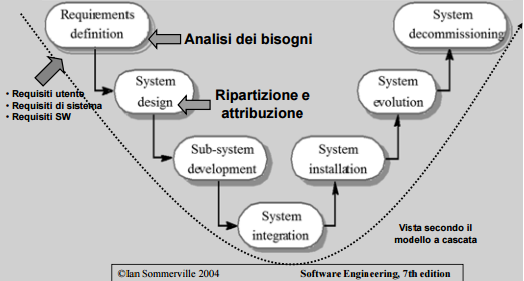
\includegraphics[width=0.75\columnwidth]{img1.png}
\begin{itemize}
	\item \textbf{P:} pianifico gli obbiettivi, cosa deve essere realizzato, come andrà controllato;
	\item \textbf{D:} do;
	\item \textbf{C:} controllo dove sono arrivato rispetto a quello che avevo pianificato.
\end{itemize}


Non ci interessa la burocrazia, ma strumenti che ci aiutino a fare bene il nostro lavoro e ad avere un approccio più strutturato. L'attenzione alla qualità deve spostarsi dal prodotto al \textbf{sistema} e alla sua organizzazione. La qualità di prodotto è meno importante della qualità di sistema. Il sistema è un insieme di attività organizzate e coese.
Nel caso del \textbf{Ciclo di Deming} pianifico attività che producono miglioramenti. Tutti i processi hanno come prima attività l'istanziazione del processo e poi la pianificazione. Per poter migliorare devo prima misurare, e controllare il miglioramento avvenuto.

\textbf{Modello di qualità:} rappresentazione astratta, insieme di strumenti che servono a valutare la qualità.\\ 
\textbf{Modello di Bohem:} la qualità viene descritta da un insieme di caratteristiche fissate e non arbitrarie. Bohem ne ha definite 7 e le ha suddivise in ulteriori 15 sotto categorie. Secondo ISO/IEC 9126:2001, che è un'evoluzione di Bohem, ho i seguenti principi:

\begin{enumerate}

	\item \textbf{Funzionalità:} avere le funzionalità attive è qualità;
	\item \textbf{Affidabilità};
	\item \textbf{Efficienza:} devo metterci poco tempo, quante risorse uso per fare una determinata cosa;
	\item \textbf{Usabilità:} non vanno bene cose troppo complesse per gli utilizzatori;
	\item \textbf{Manutenibilità};
	\item \textbf{Portabilità}.

\end{enumerate}

La \textbf{qualità in uso} è una dimensione specifica rivolta esclusivamente all'utente finale. Ho queste caratteristiche:

\begin{itemize}

	\item \textbf{Efficace};
	\item \textbf{Produttività:} lo strumento mi fa andare più veloce;
	\item \textbf{Soddisfazione:};
	\item \textbf{Portabilità}.
	
\end{itemize}

\textbf{Software metrics:} qualsiasi tipo di misura che riguarda un sistema software, un processo o la documentazione. Questo fa si che abbia prodotti e processi valutabili

\end{document}
